%%%%%%%%%%%%%%%%%%%%%%%%%%%%%%%%%%%%%%%%%
% Structured General Purpose Assignment
% LaTeX Template
%
% This template has been downloaded from:
% http://www.latextemplates.com
%
% Original author:
% Ted Pavlic (http://www.tedpavlic.com)
%
% Note:
% The \lipsum[#] commands throughout this template generate dummy text
% to fill the template out. These commands should all be removed when
% writing assignment content.
%
%%%%%%%%%%%%%%%%%%%%%%%%%%%%%%%%%%%%%%%%%

%----------------------------------------------------------------------------------------
%	PACKAGES AND OTHER DOCUMENT CONFIGURATIONS
%----------------------------------------------------------------------------------------

\documentclass{article}

\usepackage{fancyhdr} % Required for custom headers
\usepackage{lastpage} % Required to determine the last page for the footer
\usepackage{extramarks} % Required for headers and footers
\usepackage{graphicx} % Required to insert images
\usepackage{natbib} % bibliography
\usepackage{filecontents}
\usepackage{pgfplots}
\usepackage{pgfplotstable}
\usepackage{siunitx}
\usepackage{float}
\usepackage{tikz}
\usepackage{tikz-uml}
\usetikzlibrary{backgrounds,arrows,automata}
\usepackage{colortbl}
\pgfplotsset{compat=1.5}
\usepackage[latin1]{inputenc}

% Margins
\topmargin=-0.45in
\evensidemargin=0in
\oddsidemargin=0in
\textwidth=6.5in
\textheight=9.0in
\headsep=0.25in

\linespread{1.1} % Line spacing

% Set up the header and footer
\pagestyle{fancy}
\lhead{\hmwkClass:\ \hmwkTitle} % Top left header
\chead{} % Top center header
\rhead{\firstxmark} % Top right header
\lfoot{\lastxmark} % Bottom left footer
\cfoot{} % Bottom center footer
\rfoot{Page\ \thepage\ of\ \pageref{LastPage}} % Bottom right footer
\renewcommand\headrulewidth{0.4pt} % Size of the header rule
\renewcommand\footrulewidth{0.4pt} % Size of the footer rule

\setlength\parindent{0pt} % Removes all indentation from paragraphs

%------------------------------------------------------------------------------
%	DOCUMENT STRUCTURE COMMANDS
%	Skip this unless you know what you're doing
%------------------------------------------------------------------------------

% Header and footer for when a page split occurs within a problem environment
\newcommand{\enterSectionHeader}[1]{
\nobreak\extramarks{#1}{#1 continued on next page\ldots}\nobreak
\nobreak\extramarks{#1 (continued)}{#1 continued on next page\ldots}\nobreak
}

% Header and footer for when a page split occurs between problem environments
\newcommand{\exitSectionHeader}[1]{
\nobreak\extramarks{#1 (continued)}{#1 continued on next page\ldots}\nobreak
\nobreak\extramarks{#1}{}\nobreak
}

\newcommand{\mainSectionName}{}
\newenvironment{mainSection}[1]{
\renewcommand{\mainSectionName}{#1}
\pagebreak
\section{\mainSectionName}
\enterSectionHeader{\mainSectionName} % Header and footer within the environment
}{
\exitSectionHeader{\mainSectionName} % Header and footer after the environment
}

\newcounter{httpTableCounter}
\newcommand{\httpTable}[5]{
  \stepcounter{httpTableCounter}
  \begin{figure}[H]
    \begin{center}
      \begin{tabular}{|l|r|r|}
        \hline
        \multicolumn{3}{ |c| }{HTTP Response Codes for \texttt{m3.#1}}\\
        \hline
        Code & Highest Rate & Total \\
        \hline
        200  & #2/sec  & #3 \\
        503  & #4/sec  & #5 \\
        \hline
      \end{tabular}
      \caption{Please note this table only includes \texttt{200} and
      \texttt{503} response codes.}
      \label{fig:http#1}
    \end{center}
  \end{figure}
}

%------------------------------------------------------------------------------
%	NAME AND CLASS SECTION
%------------------------------------------------------------------------------

\newcommand{\hmwkTitle}{Market Chirp} % Assignment title
% \newcommand{\hmwkDueDate}{Monday,\ January\ 1,\ 2012} % Due date
\newcommand{\hmwkClass}{ABCs} % Course/class
\newcommand{\hmwkAuthorName}{Alex Fong, Brandon Woo, Chris Konstad, Sakib Shaikh}

%------------------------------------------------------------------------------
%	TITLE PAGE
%------------------------------------------------------------------------------

\title{
\vspace{2in}
\textmd{\textbf{\hmwkClass:\ \hmwkTitle}}\\
\vspace{3in}
}

\author{\textbf{\hmwkAuthorName}}
\date{December 3rd, 2015}

%------------------------------------------------------------------------------
% Bibliography
\begin{filecontents*}{ABCs.bib}
@MISC{GitBranching,
  author = {{Keith D. Gregory}},
  title = {{Practical Git: A Workflow to Preserve Your Sanity}},
  note = {[Online; accessed Nov 30, 2015]},
  url = {http://www.kdgregory.com/images/scm.git/02-fishbone.gif}
}
\end{filecontents*}
%------------------------------------------------------------------------------

%------------------------------------------------------------------------------
% USER ARRIVAL RATES
\begin{filecontents}{users.temp}
X,Y
0,1
30,2
60,4
90,8
120,16
150,32
180,64
210,128
240,256
270,512
\end{filecontents}
%------------------------------------------------------------------------------

\begin{document}

\maketitle

%------------------------------------------------------------------------------
%	TABLE OF CONTENTS
%------------------------------------------------------------------------------

\newpage
\tableofcontents
\newpage

%------------------------------------------------------------------------------
%	PROBLEM 1
%------------------------------------------------------------------------------

% To have just one problem per page, simply put a \clearpage after each problem

%\begin{homeworkProblem}
\begin{mainSection}{Introduction}
Market Chirp is a stock recommendation web application developed in the context
of UCLA CS 188/219, Scalable Internet Services in Fall 2015 by the team ABCs.
The application analyzes Twitter's sentiment on all NASDAQ stocks and provides
the user with the information required to make sound investment decisions.
\\

\subsection{What we do}
\indent Market Chirp provides users with an interface to quickly get historical
and current data for any given stock. Market Chirp's defining feature is
providing sentiment analysis of the stock based on influential and recent
tweets so users gain valuable insight on what others are saying about the
company performance. We provide users a platform to make a portfolio of their
favorite companies and monitor their stock market performance.
\\
\begin{figure}[h]
  \centering
  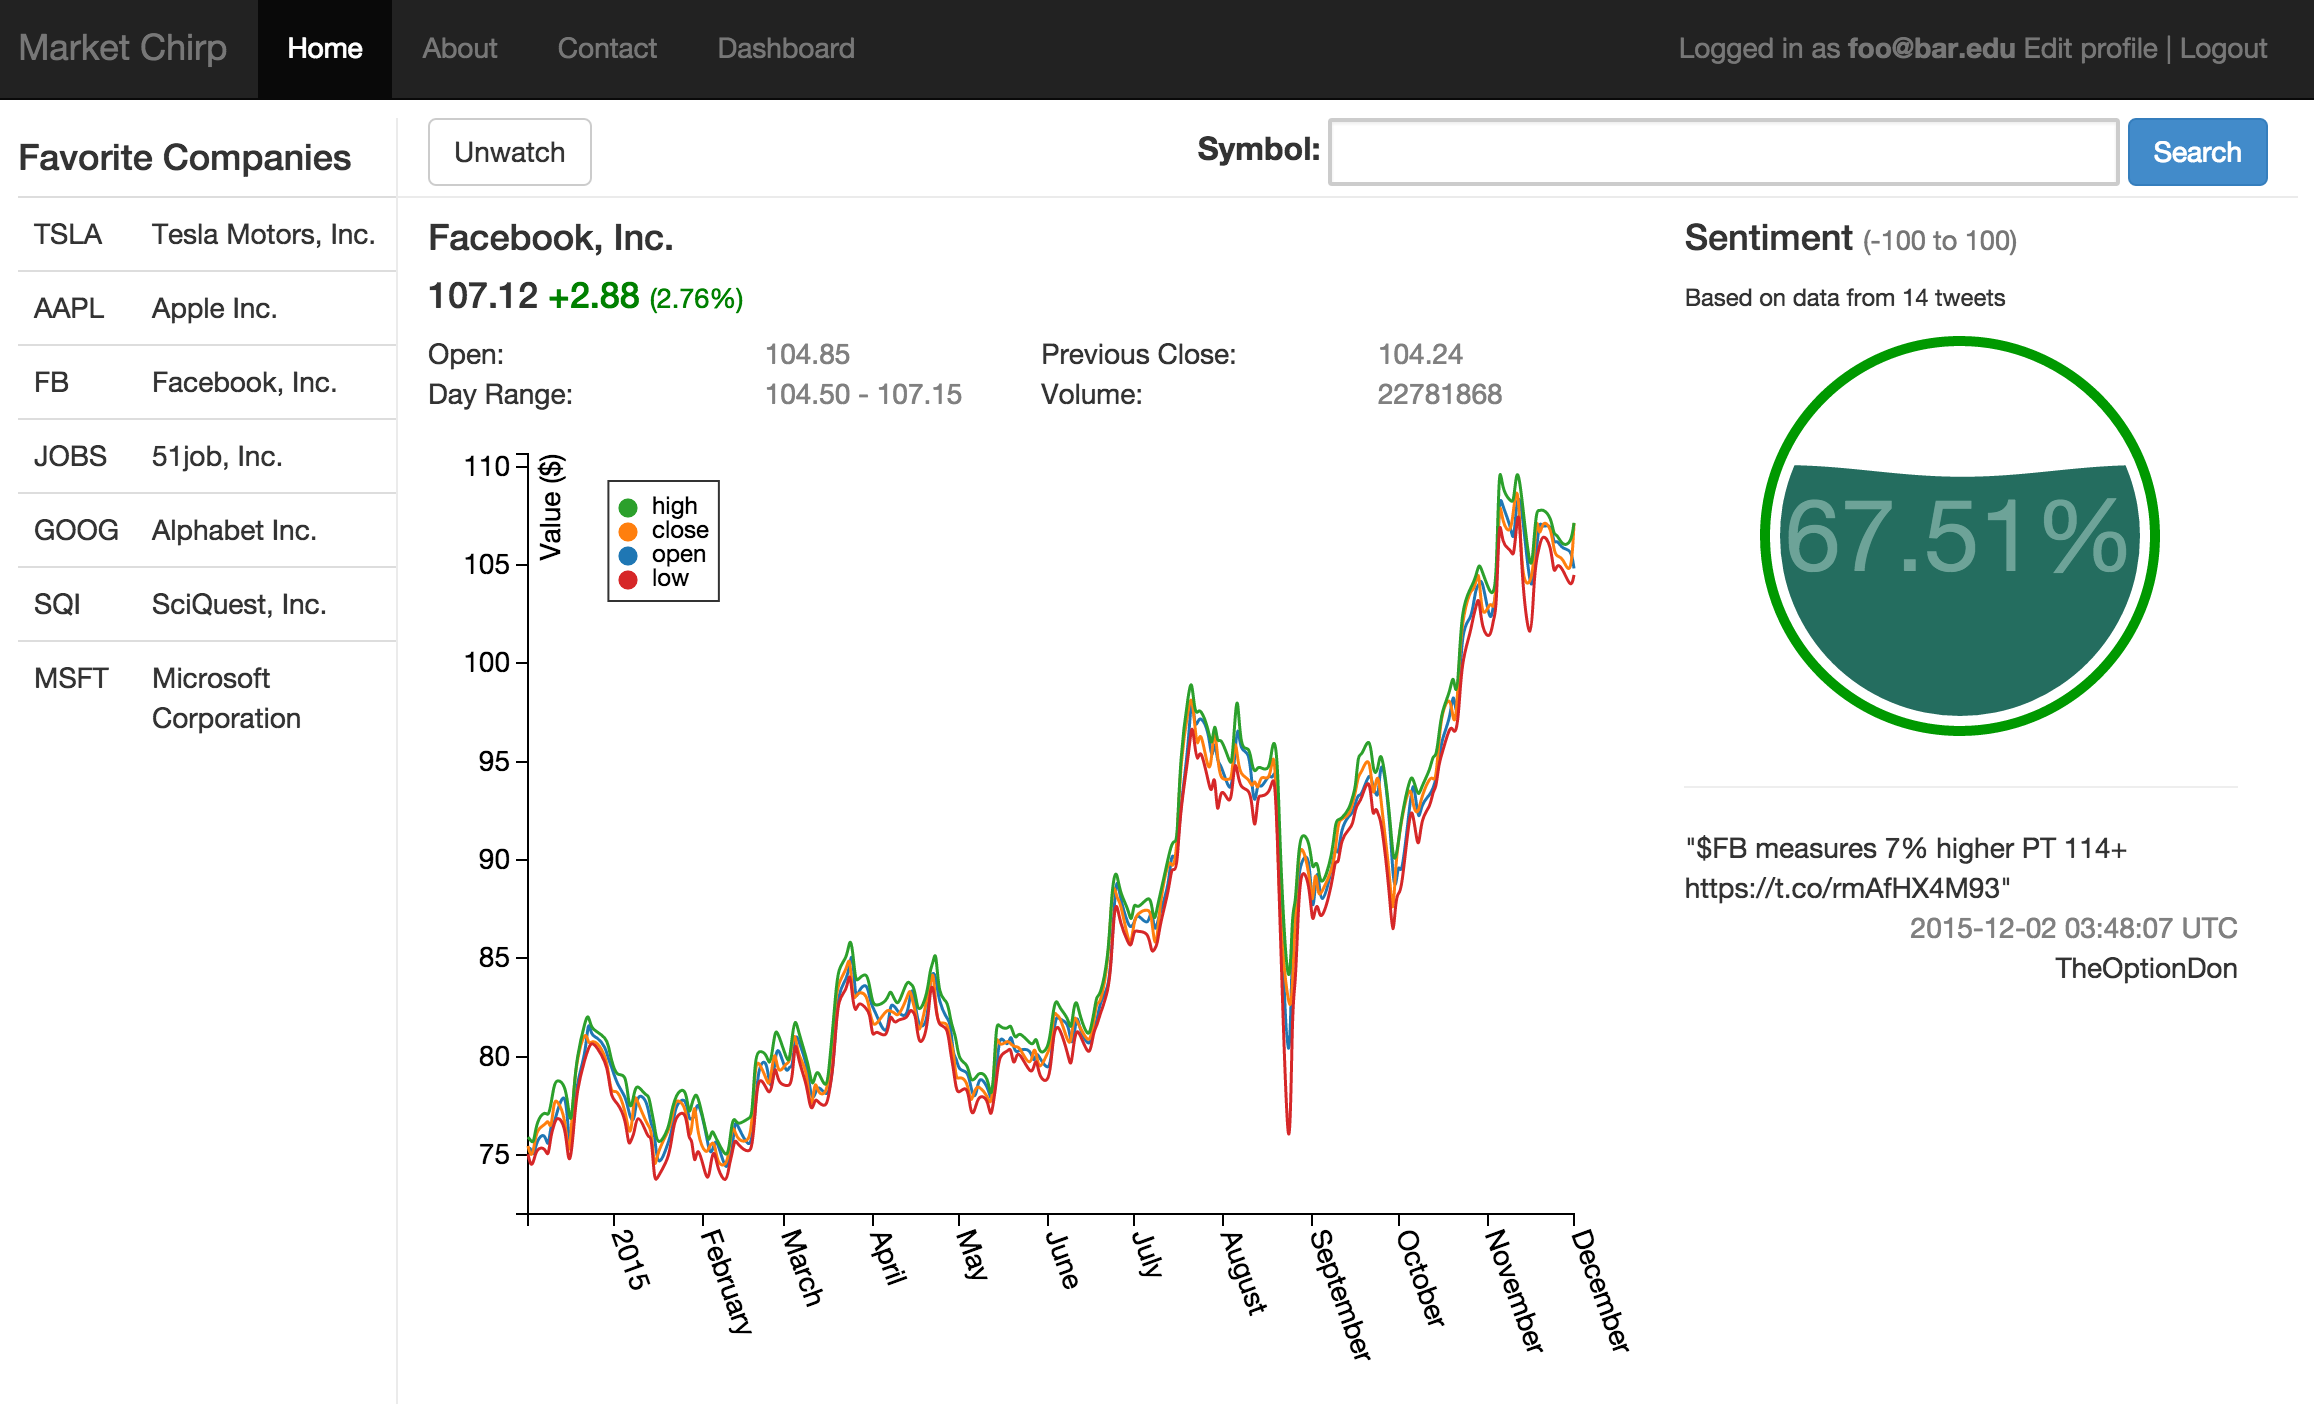
\includegraphics[width=1\columnwidth]{resources/dashboard.png} % Example image
  \caption{Example dashboard containing stock history, sentiment, and
  favorites.}
  \label{fig:dashboard}
\end{figure}

\subsection{Our goal}
The goal of Market Chirp is to quickly analyze the public's opinion of
high-quality stocks through short notes on Twitter. Since the feed of Tweets is
queried in real time when a user searches for a certain stock, the sentiment
analysis of a stock represents the public's current opinion of whether a stock
is bullish or bearish. For example, if a stock's market price is on a downhill
trend but its Twitter sentiment is on an uptrend, one may take that as an
indication to buy the stock. This is because the temperature of a company in
the eye of the public is often a good indicator of their stock's future
performance on the market. Market Chirp's ultimate goal is not to predict the
prices of the whole of the stock market, as the sentiment is based on a limited
data set of people tweeting about a stock, but to give a recommendation of
whether to buy the stock or not stock based on the public's opinion.
\\
\subsection{How we do it}
Market Chirp is implemented in Ruby on Rails (Ruby 2.2.1 and Rails 4.2.4). The
back end data store is a relational database management system, in our case
MySQL. Since the purpose of CS 188/219: Scalable Internet Services is to build
and deploy a scalable web service, this report will therefore discuss the
deployment, performance and scalability of Market Chirp.
\end{mainSection}

\begin{mainSection}{Development Process}
\begin{figure}[h]
  \centering
  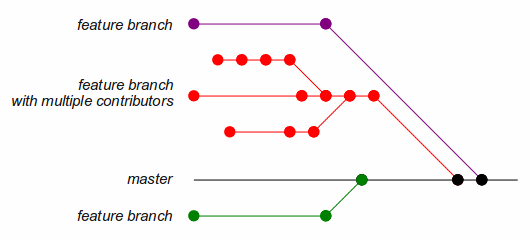
\includegraphics[width=0.75\columnwidth]{resources/git.jpg} % Example image
  \caption{Example of our Git branching technique (\cite{GitBranching})}
  \label{fig:git}
\end{figure}

\subsection{Planning}
Through the development of Market Chirp, our team used an Agile framework. We
had weekly sprint planning meetings to discuss where the project was headed
along with retrospective meetings to gain a perspective on what we had
accomplished or still had yet to implement over the past week. Tasks not
completed by the specified sprint date were automatically moved into a backlog
or icebox in order to be completed in future sprints. By using these stand-up
meetings, our team was able to precisely figure out the tasks that needed to be
finished and how our individual features were pushed into the big picture of
the entire product and its scalability. These meetings also served to keep us
on track and figure out how all the features we were developing would interact.
\\

\subsection{Scheduling}
Pivotal Tracker guided us in following the Agile development framework. With
Pivotal Tracker integrated with GitHub to keep track of certain features or
issues, our commits and releases could be synced up to reflect the current
status of the application. We were able to assign tickets to certain people in
order to split the work up in an efficient manner. By modularizing the tasks,
implementing the features and fixing bugs became much smoother than using
another development framework such as Waterfall Planning. As the quarter moved
along however, our use of Pivotal Tracker slowly faded out as we kept in
constant contact with each other and remained up date to with our progress on
the project.
\\

\subsection{Automated testing}
Since Rails is a test driven development framework, it automatically created
testing templates for the classes we developed. We made sure to follow test
driven development in which one creates test cases for a feature before
actually implementing the feature. By following TDD, edge cases were covered as
we programmed out the features since we thought about what they were
beforehand. Since we created ample test cases, the majority of our code was
covered and allowed us to be confident our website would not crash when scaled
upward.
\\

Travis CI was set up as a continuous integration service for building and
testing the project. We created numerous test cases that would be run each
commit to verify the version control's reliability. Connecting Travis CI to
GitHub allowed us to keep committing new code, while at the same time testing
its reliability and keeping it bug free.
\\

To further minimize the bugs in our code and to follow the D.R.Y. practices, we
ran RuboCop and Pre-commit before our commits. RuboCop is a Ruby static code
analyzer that enforces many of the guidelines outlined in the community created
Ruby Style Guide. This linter analyzed all of the code in our repository and
provided metrics that ensured our Ruby code was stylistically accurate. Before
we committed our code, Git fired off a Pre-commit hook that ran RuboCop. If
RuboCop returned any warnings on our code, our code could not be committed.
Thus, our code was ensured to be up-to-date with the current stylistic
guidelines.
\\
\subsection{Version control}
Our version control management system was Git. By keeping the master branch as
our production branch, our releases on AWS were always in sync with the latest
release on our remote GitHub. We all worked on separate branches and used pull
requests to merge our new code into the other branches eventually merging into
master. By constantly rebasing our branches, our development history is clean
and looks as though only one person had developed it. Separating the features
and bug fixes into their own respective branch allowed each developer to focus
on his own feature without conflicting with other developers. After merging in
the features, the application's version control was clean.

\subsection{Pair programming}
We also performed pair programming in certain scenarios such as the development
of our Memcached server side caching optimization. Pair programming allowed us
to minimize the errors in our code since we had multiple eyes on the screen at
a time. One person could focus on hashing out the code while the other checked
for syntactic or logical errors. In doing so, the time from the outlining of a
feature to pushing production ready code was optimized and we were able to save
a substantial amount of time.

\subsection{Important Gems Used For Development}
We utilized several important rails gems that helped make the development of
our application much easier. The gems listed below added important
functionality such as user management and wrappers for APIs. Using the gems is
better practice because it saves development time as we do not have to
implement and debug code in house. These functionality provided in external
gems is more robust and has been tested.

The gems we used include:
  \begin{enumerate}
    \item \textbf{devise}: gem is a MVC based authentication solution for
      rails. It is flexible and can be easily customized based on individual
      requirements.
    \item \textbf{sentimentalizer}: gem provides an implementation to run
      sentiment analysis on a block of texts. We integrated this gem manually
      instead of using a gem file. We made this design decision to improve the
      quality of the sentiment analysis by passing custom training data
      consisting of manually scraped and labeled stock market tweets. This
      enabled the sentiment analyzer to better recognize stock market terms.
    \item \textbf{twitter}: gem provides a clean interface to the Twitter API.
    \item \textbf{yahoofinance}: gem provides a clean interface to the Yahoo
      Finance API for stock and historical data
    \item \textbf{d3-rails}: gem provides the D3 library to create plots and
      graphs
  \end{enumerate}

\end{mainSection}
\pagebreak

\begin{mainSection}{Application}
  \subsection{Application Architecture}
  Ruby on Rails' use of a MVC (Model View Controller) system allowed us to
  quickly prototype features during development, and later provided insulation
  between different aspects of our website. The user facing View provides the
  graphical interface with which they can see the result of their actions. When
  the user wants to interact with the application, say by submitting a form or
  searching for a stock, they are using a Controller. Lastly there is the Model
  which takes instructions from the Controller and updates the user's View. The
  Model also interacts with our application's database, in our case by keeping
  track of favorite stocks and cached data.
  \\
  \begin{figure}[H]
  \begin{center}
      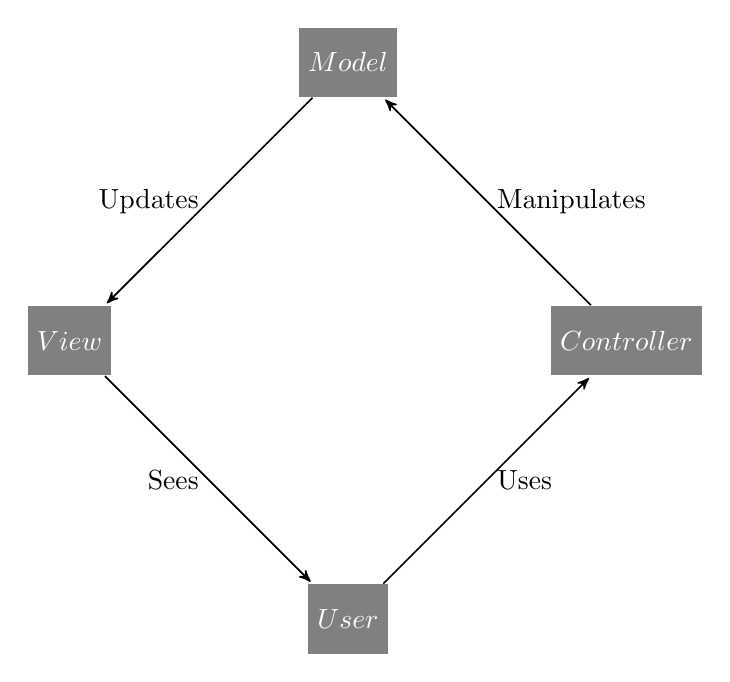
\begin{tikzpicture}[->,>=stealth',shorten >=1pt,auto,node distance=5cm,
                          semithick]
        \tikzstyle{every state}=[rectangle,fill=gray,draw=none,text=white]

        \node[state] (A)                    {$View$};
        \node[state] (B) [above right of=A] {$Model$};
        \node[state] (D) [below right of=A] {$User$};
        \node[state] (C) [below right of=B] {$Controller$};

        \path (B) edge              node [left] {Updates} (A)
              (C) edge              node [right] {Manipulates} (B)
              (D) edge              node [right] {Uses} (C)
              (A) edge              node [left] {Sees} (D);
      \end{tikzpicture}
    \end{center}
    \caption{Graphical interface of a Model View Controller Architecture}
    \label{dig:MVC}
  \end{figure}

  \subsection{Database layout}
  \begin{figure}[H]
    \begin{tikzpicture}
      % COMPANY
      \begin{umlclass}[x=5,y=5]{Company}{symbol : varchar(5)\\name :
          varchar(255)\\sector : varchar(255)\\industry :
          varchar(255)\\created\_at : datetime\\updated\_at : datetime\\
        }{}
      \end{umlclass}
      % FAVORITE_COMPANY
      \begin{umlclass}[x=0,y=0]{Favorite\_Company}{user\_id :
          foreign\_key\\company\_id : foreign\_key\\active :
          boolean\\created\_at : datetime\\updated\_at : datetime
        }{}
      \end{umlclass}
      % USER
      \begin{umlclass}[x=11,y=0]{User}{email :
          varchar(255)\\encrypted\_password :
          varchar(255)\\reset\_password\_token :
          varchar(255)\\reset\_password\_sent\_at :
          datetime\\remember\_created\_at : datetime\\sign\_in\_count :
          int(4)\\current\_sign\_in\_at : datetime\\last\_sign\_in\_at :
          datetime\\current\_sign\_in\_ip : varchar(255)\\last\_sign\_in\_ip :
          varchar(255)\\created\_at : datetime\\updated\_at : datetime
        }{}
      \end{umlclass}
      % FINANCE_CACHE
      \begin{umlclass}[x=0,y=10]{Finance\_Cache}{hist\_data :
          varchar(65535)\\curr\_data : varchar(65535)\\category :
          int(4)\\company\_id : foreign\_key\\created\_at :
          datetime\\updated\_at : datetime
        }{}
      \end{umlclass}
      % SENTIMENT_CACHE
      \begin{umlclass}[x=11,y=10]{Sentiment\_Cache}{tweet\_when :
          datetime\\score : decimal\\tweet\_text : varchar(255)\\tweet\_author
          : varchar(255)\\num\_tweets : int(4)\\company\_id :
          foreign\_key\\created\_at : datetime\\updated\_at : datetime
        }{}
      \end{umlclass}
      \umluniassoc[geometry=|-|]{Company}{Favorite\_Company}
      \umluniassoc[geometry=|-|]{Finance\_Cache}{Company}
      \umluniassoc[geometry=|-]{Sentiment\_Cache}{Company}
      \umluniassoc[geometry=|-|]{User}{Favorite\_Company}
    \end{tikzpicture}
    \caption{Diagram of the database tables and how they are connected.}
    \label{fig:database_layout}
  \end{figure}

  \begin{figure}[H]
    \begin{tabular}{|p{4cm}|p{11.51cm}|}
      \hline
      \textbf{Model} & \textbf{Purpose}\\
      \hline
      \rowcolor[gray]{.9}
      Company & This table contains the non-financial information about the company.  It is what matches a stock symbol to a complete company name, and other information about the company.\\
      Favorite Company & This table is what links a User to the companies that they favorited.\\
      \rowcolor[gray]{.9}
      Finance Cache & This table stores the data received from Yahoo! Finance so we can reduce third-party API hits.\\
      Sentiment Cache & This table stores the sentiment data calculated from the data received from Twitter so we can both reduce third-party API hits and greatly improve performance.\\
      \rowcolor[gray]{.9}
      User & This table stores User account data.\\
      \hline
    \end{tabular}
    \caption{Table of Market Chirp's models and their purposes.}
    \label{fig:database_description}
  \end{figure}
\end{mainSection}

\begin{mainSection}{Testing}
  \subsection{Server configuration}
  We used the following software packages for the deployment of the production
  version of our application:
  \begin{itemize}
    \item NGINX
    \item Phusion Passenger
    \item MySQL
  \end{itemize}

  We modified the provided cloud formation template's JavaScript Object
  Notation (JSON) files to configure our server with the proper environmental
  variables, letting us keep our secret keys out of our public version
  control.\\

  The service was developed on our personal laptops, with all performance
  testing running on Amazon Web Services (AWS).  It was trivial for us to
  deploy new versions because we only had to deploy for performance testing,
  which was handled by our server provisioning scripts.\\

\begin{figure}[H]
  \begin{center}
    \begin{tabular}{| l | r | r | r | }
      \hline
      \multicolumn{4}{ |c| }{M3 Server Configurations}\\
      \hline
      Server Size & Cores & RAM (GiB) & Process Parallelization\\
      \hline
      Med     & 1 &  3.75 & 1 \\
      Large   & 2 &  7.50 & 2 \\
      XLarge  & 4 & 15.00 & 4 \\
      2XLarge & 8 & 30.00 & 8 \\
      \hline
    \end{tabular}
    \caption{Table of server configurations.  These settings were used for all
    tests.  For a server with $n$ cores, $n$ worker processes were used.  Each
  worker process was single threaded. By minimizing differences in the testing
setups, we were able to clearly show the effects of each optimization.}
    \label{tab:m3}
  \end{center}
\end{figure}

When separate database servers were used (for example, in horizontal scaling),
the database server was the same size as the application server
(\texttt{db.m3med} was used for \texttt{m3.med}).\\

After analyzing our common queries, we added indices to our database to
improve read performance.  These indices reduced query time for reads,
improving database performance for our most common operation.\\

  \subsection{User simulation}
  \begin{figure}[H]
    \begin{center}
      \begin{tikzpicture}
        \begin{axis}[title=Test User Arrival Rates,
            xlabel = Time (sec),
            ylabel = Users/sec,
            legend pos = outer north east,
          ]
          \addplot[thick, orange] table [
              col sep=comma,
              x = X,
              y = Y,
            ] {users.temp};
        \end{axis}
      \end{tikzpicture}
    \end{center}
    \caption{Graph showing the number of test users sent from our Tsung server
    to our application server throughout the duration of the performance
  tests.}
    \label{graph:users}
  \end{figure}

  Our Tsung tests used the test user arrival rates shown in Figure
  \ref{graph:users}. A tabulation of the phases of users arrival rates can be
  seen below.\\

\begin{figure}[H]
  \begin{center}
    \begin{tabular}{| c | c | c | c | c | c | c | c | c | c | c |}
      \hline
      \multicolumn{11}{ |c| }{10 Phases of user arrivals}\\
      \hline
       Phase Number & 1 & 2 & 3 & 4 & 5 & 6 & 7 & 8 & 9 & 10\\
      \hline
      New users per second & 1 & 2 & 4 & 8 & 16 & 32 & 64 & 128 & 256 & 512\\
      \hline
    \end{tabular}
  \end{center}
  \caption{Table listing the number of users arriving per second during each
  phase of the test.}
\end{figure}

  Missing our slowest level of caching, our MySQL "caches" of Twitter sentiment
  data, and to a lesser extent Yahoo! Finance data, causes $20+$ second delays.
  Because of these unreasonably long delays, our service would have worker
  processes keeping those caches warm if we deployed this to the real world.
  To simulate this effect in our tests, we limited our test users to
  interacting with a small subset of the real world stocks and we warmed up the
  cache before running the tests.  According to our tests, users only care
  about Apple, Facebook, Google and Tesla stocks, which, while unrealistic, is
  a useful simulation for comparing performance tests.  Another benefit of
  focusing on popular stocks is that we are guaranteed to always have enough
  Twitter data about each stock symbol.  Some of the less popular stock symbols
  would have 5 tweets or less, making both the data inaccurate and the request
  too easy to strain the system.\\


  \subsection{Critical Path}
  Our critical path through our application was the path that we thought the
  average user was most likely to hit.  We had two user models, with a 50\%
  chance that either model was selected for each test user:
  \begin{enumerate}
    \item A user who is not logged in
    \item A user who is logged in
  \end{enumerate}

  While visiting each page, the test user would wait a randomized amount of
  time up to a threshold to emulate a person either looking at the page or
  filling out forms.

  \subsubsection{User not logged in}
  A user who is not logged in has no account on Market Chirp and therefore has
  no favorites.  They are also unable to access the Dashboard feature, which is
  the page that requires the most data fetching and handling, making it the
  most expensive page to load.  Instead, this user:
  \begin{enumerate}
    \item Visits our homepage
    \item Visits our sentiment analysis page
    \item Searches for FB
    \item Searches for AAPL
    \item Searches for GOOGL
    \item Searches for TSLA
    \item Visits our stock data page
    \item Searches for FB
    \item Searches for AAPL
    \item Searches for GOOGL
    \item Searches for TSLA
  \end{enumerate}

  \subsubsection{User is logged in}
  A logged in user would want to check their favorited stocks, which is most
  easily done through the Dashboard page.  From there, we thought the average
  user would check their stocks, look for a new one, favorite the new stock and
  drop one of their favorited stocks.  This user:
  \begin{enumerate}
    \item Logs in
    \item Visits their dashboard
    \item Visits the dashboard for GOOGL
    \item Favorites GOOGL
    \item Visits the dashboard for TSLA
    \item Visits the dashboard for FB
    \item Visits the dashboard for AAPL
    \item Removes AAPL from their favorite list
    \item Logs out
  \end{enumerate}

  \subsection{Initial testing}
  The first tests of Market Chirp showed massive performance issues.  Twitter
  sentiment data was calculated for all 100 tweets (pulled from Twitter
  separately for each request), leading to $20+$ second delays in getting
  results when searching for a stock symbol. During this period, the web page
  was unresponsive to the user and appeared to be frozen. From looking at the
  logs and \texttt{top}, it was clear that the process was CPU bound.  No
  formal Tsung testing happened at this performance level because individual
  page loads took too long and the service was not ready for even a single
  user.\\

  A MySQL driven "cache" was created to store Twitter analysis for a day, for
  each stock that was searched.  While initial stock searches caused
  unreasonable delays of $20+$ seconds, subsequent delays were much, much
  smaller, happening in less than $5$ seconds.  The cache stores the overall
  calculated sentiment and the single tweet out of the $100$ sampled tweets
  that has the closest sentiment value as an average tweet for the given
  sample.\\

  A similar MySQL driven caching system was added to cache the 10 years of
  Yahoo! Finance stock data downloaded and current stock data for each symbol
  requested.  The stock data itself was stored as a JSON text blob, as the
  client side graphing library read in that JSON.  It made more sense to store
  the JSON received from Yahoo! Finance in the same format that the graph
  required, than it did to parse the JSON, store each value individually, and
  read those values out as JSON later.

  \subsection{Vertical scaling}
  Vertical scaling, simply throwing more processing power at the problem, is
  simple but expensive.  We expected to get marginal performance gains by
  scaling vertically because our main bottleneck was the CPU bound Twitter
  sentiment analysis. To test the response of our application to an increasing
  load when equipped with more raw power, we set up a number of instances of
  increasing size. We chose the M3 family of instances to test on as they gave
  a nice balance of computational capabilities, memory, and network resources.

  \subsubsection{Performance graph}
  \begin{figure}[H]
    \begin{center}
      \begin{tikzpicture}
        \begin{axis}[title=Vertical Scaling,
            xlabel = Time (sec),
            ylabel = Users/sec,
            legend pos = outer north east,
          ]
          \addplot[thick, orange] table [
              col sep=comma,
              x = X,
              y = Y,
            ] {resources/m3med/data/200.csv};
          \addplot[thick, blue] table [
              col sep=comma,
              x = X,
              y = Y,
            ] {resources/m3large/data/200.csv};
          \addplot[thick, green] table [
              col sep=comma,
              x = X,
              y = Y,
            ] {resources/m3xlarge/data/200.csv};
          \addplot[thick, magenta] table [
              col sep=comma,
              x = X,
              y = Y,
            ] {resources/m32xlarge/data/200.csv};
          \addlegendentry{M3 Med}
          \addlegendentry{M3 Large}
          \addlegendentry{M3 XLarge}
          \addlegendentry{M3 2XLarge}
          \end{axis}
        \end{tikzpicture}
      \end{center}
      \caption{Graph of performance during vertical scaling.}
      \label{graph:vertical}
    \end{figure}

    Figure \ref{graph:vertical} shows the result of our vertical scaling. As
    expected, when double the processing power was thrown at the problem, the
    number of users processed per second roughly doubled.

    \subsubsection{HTTP response statistics}
    \httpTable{Med}{1.1}{26}{140.4}{22276}
    \httpTable{Large}{9.6}{3007}{134.9}{31375}
    \httpTable{XLarge}{18.4}{5299}{127.1}{24098}
    \httpTable{2XLarge}{30.8}{7210}{123.4}{26659}

  \subsection{Horizontal scaling}
  For horizontal scaling, we moved from a single server that handled both the
  application server and the database to a network of servers (Figure
  \ref{graph:horizontal}).  This network contained an elastic load balancer
  (LB), two application servers (S0 and S1) and a MySQL server (DB).  This is a
  fairly standard horizontal scaling technique that makes it easy to increase
  the number of application servers dynamically (a side benefit of this is that
  each application server can be small, cheap, and reliable as a new server
  can be spun up to take its place if it fails).

  \subsubsection{Network diagram}
  \begin{figure}[H]
    \begin{center}
      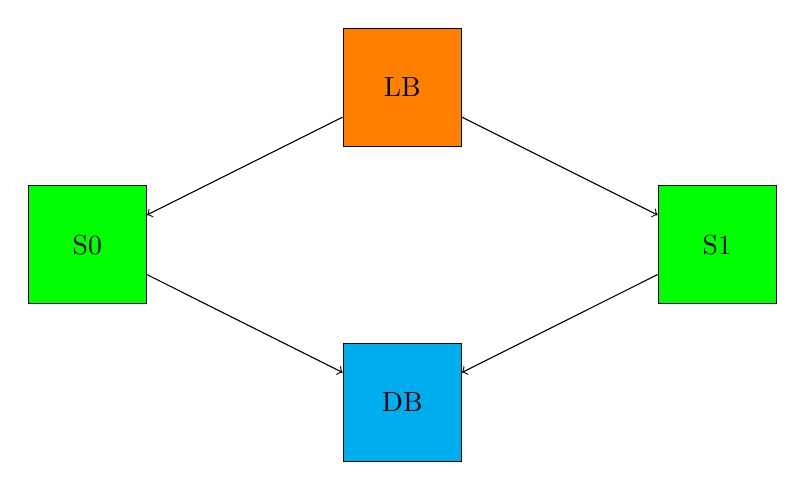
\begin{tikzpicture}[every node/.style={rectangle, fill=green,minimum
        width=15mm, minimum height=15mm,draw}]
        \node[fill=orange] (lb) at (0,0) {LB};
        \node (s0) at (-4,-2) {S0};
        \node (s1) at (4,-2) {S1};
        \node[fill=cyan] (db) at (0,-4) {DB};

        \begin{scope}[on background layer]
          \draw[->] (lb) edge (s0);
          \draw[->] (lb) edge (s1);
          \draw[->] (s0) edge (db);
          \draw[->] (s1) edge (db);
        \end{scope}
      \end{tikzpicture}
    \end{center}
    \caption{Network of Load Balancer, Servers, and Database Server}
    \label{dig:horizontal}
  \end{figure}
  Figure \ref{dig:horizontal} shows the configuration of our load balancer,
  servers and database.  This method of scaling lets us easily add more
  application servers to increase our available processing power, while not
  having to deal with distributed databases or more complex data persistence
  layers (although we are able to improve the data persistence layer if we
  want).\\

  \subsubsection{Performance graph}
  \begin{figure}[H]
    \begin{center}
      \begin{tikzpicture}
        \begin{axis}[title=Horizontal Scaling,
            xlabel = Time (sec),
            ylabel = Users/sec,
            legend pos = outer north east,
          ]
          \addplot[thick, orange] table [
              col sep=comma,
              x = X,
              y = Y,
            ] {resources/multi_m3med/data/200.csv};
          \addplot[thick, blue] table [
              col sep=comma,
              x = X,
              y = Y,
            ] {resources/multi_m3large/data/200.csv};
          \addplot[thick, green] table [
              col sep=comma,
              x = X,
              y = Y,
            ] {resources/multi_m3xlarge/data/200.csv};
          \addplot[thick, magenta] table [
              col sep=comma,
              x = X,
              y = Y,
            ] {resources/multi_m32xlarge/data/200.csv};
          \addlegendentry{M3 Med}
          \addlegendentry{M3 Large}
          \addlegendentry{M3 XLarge}
          \addlegendentry{M3 2XLarge}
          \end{axis}
        \end{tikzpicture}
      \end{center}
      \caption{Graph of performance during horizontal scaling.}
      \label{graph:horizontal}
    \end{figure}
    Figure \ref{graph:horizontal} shows the result of our horizontal scaling.
    As expected, when double the amount of servers were thrown at the problem,
    the number of users processed per second doubled.  Unlike vertical scaling,
    horizontal scaling is essentially limitless, and is usually cheaper.

    \subsubsection{HTTP response statistics}
    \httpTable{Med}{7.8}{3604}{1289.2}{196116}
    \httpTable{Large}{18.7}{3913}{1386.5}{85398}
    \httpTable{XLarge}{35}{7001}{1372.7}{80826}
    \httpTable{2XLarge}{61.2}{10429}{1319.1}{60134}

    \subsubsection{Future improvements}
    We expect our database to be mostly read, with much fewer writes as users
    are likely to spend more of their time accessing stock data than they are
    favoriting or unfavoriting stocks.  Therefore, if we wanted to increase the
    performance of our data persistence layer, we would add read-only slaves
    with a write-master.  However, as seen in Section \ref{subsec:mem}, moving
    to Memcached eliminated the need for our MySQL database to cache the stock
    analysis and price data, reducing database hits.

  \subsection{In-memory caching} \label{subsec:mem}
  Another method we implemented to speed up our application was to use a memory
  object caching system. We used Memcached in our application through the
  \texttt{dalli} gem, which stores the cache in memory instead of on disk.
  Since memory provides faster access times than disk, the read and write times
  of cache fragments were reduced. In order to provide this server-side
  caching, a new instance of Memcached needed to be started within each server.
  When keys in the memory cache expired after 24 hours of inactivity, the keys
  were wiped to allow for newer updated writes. If there was still space but
  the cached item had expired, we immediately overwrote the old value with a
  current one. Memcached replaced our MySQL database as our main caching layer
  as it was faster than MySQL but had the same required functionality.\\

  We implemented Memcached on the Yahoo! Finance data, the overall sentiment,
  and the tweet which most closely reflected the sentiment of a stock.
\end{mainSection}

%------------------------------------------------------------------------------
% CONCLUSION
\begin{mainSection}{Conclusion}
  % TODO Add more items
  From the development and testing of Market Chirp, we learned a few things
  about both deploying an application and scaling it to handle the arrival of
  hundreds of concurrent visitors:
  \begin{itemize}
    \item Market Chirp scaled linearly with both more application servers and
      more processing power.  Doubling either lead to double the users served
      per second.
    \item Using MySQL to cache computationally expensive data was an
      improvement over generating the same results each time, but it was far
      inferior to using Memcached.
    \item Memcached lead to improvements in response time because it reduced
      database hits which were much slower compared to fetching from memory.
    \item Reducing third-party API calls required for page loading improved
      performance by reducing the number of times our servers had to hit a
      remote resource.
    \item Horizontal scaling is easier and cheaper to accomplish than vertical
      scaling in the long run.
    \item Horizontal scaling is also more fault tolerant compared to vertical
      scaling. In the even that a server fails, it can be easily replaced with
      a new instance.
  \end{itemize}

\end{mainSection}
%------------------------------------------------------------------------------
% BIBLIOGRAPHY
\bibliographystyle{plainnat}
\bibliography{ABCs}
%------------------------------------------------------------------------------
\end{document}
